%% *************************************************************************
%%
%% This is the PDD for the Rovers Study - Fall 2018
%%
%% This document uses IEEEtran.cls, the official IEEE LaTeX class
%% for authors of the Institute of Electrical and Electronics Engineers
%% (IEEE) Transactions journals and conferences.
%%
%% *************************************************************************

%% *************************************************************************
% LaTeX REFERENCES
% ----------------
%   Intro to LaTeX: http://www.rpi.edu/dept/arc/docs/latex/latex-intro.pdf
%   Comprehensive LaTeX symbol list: http://tug.ctan.org/info/symbols/comprehensive/symbols-a4.pdf
%% *************************************************************************

% tell \LaTeX what kind of formatting to use
\documentclass[conference]{IEEEtran} % http://www.ctan.org/pkg/ieeetran
\usepackage{blindtext} % enable placeholder text generator
\usepackage{graphicx} % enable toolbox for embedding figures and pictures
\usepackage{nomencl} % enable package for adding a list of variables and constants at the beginning, aka "nomenclature"
\usepackage{siunitx} % enable package for easily formatting units
\usepackage{hyperref} % enable package for cross-referencing figures, sections, references etc.
% how to use hyperref: http://www2.washjeff.edu/users/rhigginbottom/latex/resources/lecture09.pdf
\usepackage[T1]{fontenc} % change text encoding to make it more crisp
\usepackage{etoolbox} % enable conditionals for help text
\usepackage{booktabs} % make beautiful tables!

% initialize nomenclature package
\makenomenclature{}

% set title. choose something as descriptive and precise as possible. Descriptive > sounding cool. remember this!
\title{RIT Space Exploration Project Design Document Standard Format and Sample Content}


\author{
  % List the authors of the design document. 
  \IEEEauthorblockN{% This block is for author Names.
    Thomas~Hall\IEEEauthorrefmark{1}
  }
  \IEEEauthorblockA{% This block is for the author Affiliations, aka department and university
    RIT Space Exploration, Rochester Institute of Technology \\ %\\ starts a new line
    Rochester, N.Y. \\
    Email:
    \IEEEauthorrefmark{1}tjh2822@g.rit.edu
  }
}

% page header for pages other than cover page
\markboth{Project Design Document Standard}%
{Hall \MakeLowercase{\textit{et al.}}: RIT Space Exploration}

% Initial setup is over, start building the document itself
\begin{document}
\maketitle%
% correct bad hyphenation here, separated by spaces
\hyphenation{explor-ation}

\begin{abstract}
  Conduct a feasibility study on the design and construction of a self driving rover. A rover would be an area of space exploration completely new to SPEX, because of this there are a lot of unknowns that need to be answered before starting this project. The study would look at the talent and skills of RIT Space Exploration and answer the question: what caliber of rover are we able to make. It would employ a multidisciplinary team to cover for construction and development. The study would lean directly into a rover project in the future. The rover would be extremely promotable and would look great at Imagine RIT. 
      % The abstract is a brief summary of the design document. Typically it includes the purpose of the design document, key goals or objectives, and justifications.
\end{abstract}

\label{sec:nomenclature}
\newcommand{\nomunit}[1]{%
\renewcommand{\nomentryend}{\hspace*{\fill}#1}}
\renewcommand{\nompreamble}{}

\nomenclature{RIT}{Rochester Institute of Technology}
\nomenclature{SPEX}{RIT Space Exploration}
\nomenclature{PDD}{Project Design Document}
% Below are examples of using nomenclature for math symbols and constants or units
\nomenclature{$\dot{m}$}{Mass flow rate
  \nomunit{\,\si{\kilo\gram\per\second}}}
\nomenclature{$c$}{Speed of light
 \nomunit{\,\SI{2.9979e8}{\meter\per\second}}}
\printnomenclature{}

% The sections included here are required. Additional sections and subsections may be added as necessary.
\section{Introduction}
\label{sec:introduction}
  % The introduction is a place to give background and context before diving into the subject matter.
  % Establish context for the work you are about to propose and the main ideas of the proposition itself.

\IEEEPARstart{E}{xamples} of proper formatting, organizational techniques and content make writing Project Design Documents as easy and painless as possible.
Writing documentation such as design documents and reports is a lot of work, but it supports the continued growth of knowledge and experience in science and engineering for SPEX as a whole.
In technical research and academia, communicating one's thoughts and ideas is arguably more important than the ideas themselves.
For example, when applying to a grant from a scientific foundation, receiving funding to continue research impinges on how the motives and techniques of a research group resonate with the goals and objectives of the foundation.

In the case of SPEX, a PDD carries value in the act of documenting ideas and effectively communicating them with others within and external to RIT Space Exploration.

\section{Primary Objective}
\label{sec:primary-obj}
  % At the end of the day, whether the project ``succeeds'' or ``fails'' is judged against the objectives it sought to meet.
  % Note that results that contradict expectations/hypotheses are not failures if the scientific \& engineering methods are followed along the way.
  % Sometimes our expectations are wrong and that can be just as successful as getting data we thought we'd see.
  % What matters are what questions you intend to answer.
  % This is the main purpose or main goal the project hopes to achieve.

The goal of this study is to asses the technical ability and skills of RIT Space Exploration regarding the constuction and implementation of a mock rover. 
This study will create a plan including answering unknowns about the rover, how the rover will be built and progammed, and what skills / resourses are needed to build the afforementioned rover. 

At the end of the semester these questions will lead to a well developed PDD for the following semester.  

%\begin{figure}
%  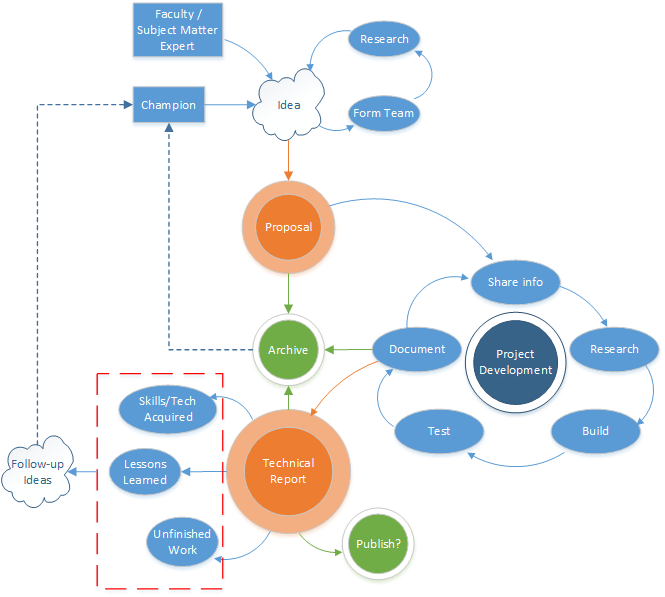
\includegraphics[width=\linewidth]{figs/project-life-cycle.png}
%  \caption{A PDD is the first piece of documentation to be archived in the project life cycle. Since the life cycle can be iterative, a new design document may also refer to one or more previous SPPs.}
%\label{fig:lifecycle}
%\end{figure}

\section{Secondary Objectives}
\label{sec:secondary-obj}
  % Secondary Objectives are lower priority or bonus objectives that are significant but not the main focus of the project. This template does not have secondary objectives.
The study will also look into the University Rover Competition (URC) as hosted by the mars Society as a potential long term goal. The competition is held annually and features 4 very intense competitions. Such a rover would need to be fully self navigating, perform scintific analysis on soil samples, and haveing a robotic arm capable of fine motor contol. Sucha project would be among the most ambitious SPEX has ever attempted. 

\autoref{tab:questions} lists questions the project will need to answer in order to make a PDD.

\begin{table*}
% this table is too wide for the two-column format, so we let it expand across both columns
% we haven't told LaTeX where to put this so it'll find the best place.
    \caption{List of questions study will answer}
    \centering
    \begin{tabular}{@{}llcc@{}}
        % READ THIS!! https://www.inf.ethz.ch/personal/markusp/teaching/guides/guide-tables.pdf
        \toprule % line on top external edge of table
        % Separate cells in a row with &, move to the next row with \\
        Question & Area \\
        \midrule % line separating two internal rows
        Will the rover design be based on something else? If so, what? & General \\
        What hardware will be present on the rover? & Hardware \\
        What type of software will be on the rover & Software \\
        How will the rover navigate terrain? & Navigation \\
        Will the rover (ever) be self driving & General \\
        What will power the rover? & Electrical \\
        How much will the rover cost? & Hardware \\
        How will the rover be funded? & General \\
        What driveterrain will the rover feature? & Locomotion \\
        How will the rover harware be tested? & Testing \\
        How will the rover software be tested & Testing \\
        Is the University Rover Challenge a possibility in the future? & Competition \\
        How will the wheels/treads word & Hardware \\
        What suspension system will the rover feature? & Hardware \\
        How can the rover be improved in the future & General \\
        How can this project be broken up into smaller sub projects? & General \\
        What will the team aim to have present ar ImagineRIT 2019? & General \\ 
        Will the rover feature and special scientific equiptment? & Hardware \\
        Do any areas of the rover design overlap with other SPEX areas? What about other clubs at RIT? & General \\
        To what spec will the rover be built? & Hardware \\
        Could RIT SPEX partner with another organization for the URC & Competition \\
        % LaTeX doesn't really like multi-line cell contents. Try to keep the text in each cell concise!
        \bottomrule
    \end{tabular}
\label{tab:questions}
\end{table*}

\section{Benefit to SPEX}
\label{sec:benefit}
% Explains the benefit to RIT SPEX

Rovers are a huge part of space exploration. It is also an area that SPEX is not currently involved with. It would be beneficial to our members to get some experience in this area.
A rover would look super good for SPEX at Imagine RIT. The rover would be rather large and would attract many eyes. We could even demo it outside if there is sufficient space. 
A rover would be very easy to get video and photos of for SPEX promotions. 
Having a rover is also another opportunity for SPEX to fundraise. There is plenty of space to place company logos on the body of the rover. It would also allow for SPEX to reach out to robotics companies.. 
The self driving component would be the heaviest computer science project SPEX would have attempted. This would help with retention of CS and SE majors. 
Machine learning and artifical intelligence are at the forefront of computer science right now. They are hevily desired in industry including space exploration.
This study would figure out the capabilities of SPEX in regards to this goal. It will also elimanate many of the unknowns and answer many of the questions at the start of a project like this. This study will create a rough plan for building such a rover.



% Subsections

\subsection{Mindset}
\label{subsec:mindset}
Firstly, it gets people in the right mindset for thinking about what is important and what needs to be considered before taking off on a project.
Publishing a PDD imbues a sense of formality that hopefully makes its way into the level of seriousness and merit that is desirable for SPEX to pursue.

\subsection{Traceability}
\label{subsec:traceability}
Similarly, a PDD serves to provide the foundation for traceability in requirements and objectives to projects as they grow and change.
This prevents blockers such as feature creep, rabbit holes, and spun tires, and hopefully prevents good projects from dying by getting too off track.

\subsection{Accessibility}
\label{subsec:plug-n-play}
  % Note below that LaTeX uses weird formatting when it comes to quotation marks.
  % The style below is correct to display forward quotes `` at the start of the phrase and backquotes '' at the end.

Having a ``plug-and-play'' template is the first step to learning how to one's own PDD\@.
It removes a major barrier of starting from scratch, providing example content to which one could refer when creating their own.
\LaTeX{} may prove to be daunting for some people, but it is arguably better to encourage people to learn LaTeX than to rely on something like Microsoft Word~\cite{lamp94}.

\section{Implementation}
\label{sec:implementation}
  % What path do you anticipate the project to take?

In the ideal case, every project begins with a design document.
That design document gets sent around to SPEX members (and non-members) to draw support and build a team.
Research and work takes place, documented along the way until  an ending point is reached (e.g.\ project completion, end of the semester, team attrition, etc.).

At the end of the project (or end of semester, whichever comes first), the team writes a report of the project with what they did, if it was successful, and recommendations for future projects.
A future SPEX member might pick up where the last paper left off, and the cycle repeats.

\subsection{Deliverables}
\label{subsec:deliverables}
  % When all is said and done, what will you have to show for it?
  % Examples: Hardware, software, poster, ImagineRIT demo, presentations, technical papers...
The primary deliverable of this study will be a PDD for the spring. It is also noted that the materials that the team will come accross or notes should also be saved in an Google Drive folder for future reference.  
The team will also present at SPEX design reviews and the weekly checkups at general meetings with the areas the team members are studying that week.
The should have a rough CAD model for the PDD showing the spacing and layout of the potential rover. The team may decide to use said CAD model to prototype. 

\subsection{Milestones}
\label{subsec:milestones}
  % Be as detailed as you can, but it's okay if there are unknowns.
  % At the very least, specify how many semester you expect the project to take until it reaches completion.
Deadlines and milestones provide clear goals from which timelines and schedules may be developed, and also set up a project for a series of ``sanity checks'' along the project's development cycle.
Early on, these milestones include design reviews on system and subsystem levels.
Later, milestones are usually important tests or experiments.
Events such as ImagineRIT may also serve as milestones to mark a project's development progress or completion.

A notional timeline is shown in \autoref{tab:short-example}.

\begin{table}[hb!]
    % the "h" in these brackets tells LaTeX to put the table Here. Try [t] for top and [b] for bottom,
    % or [hbp] for "here, or if you can't do that put it at the bottom of the page, or if you can't do that put it on its own page.
    % Here we've also used an "!" to yell at LaTeX to DO THIS OR ELSE!
    \caption{Notional timeline of Project Milestones.}
    \centering
    \begin{tabular}{@{}cll@{}}
    % the letters here ^^^^ designate the columns.
    % (l=left align, c=center, r=right align)
    % the weird @{} thingies tell LaTeX to not have left-right padding between cells
    % so cells butt up right against the edge
    \toprule
    Phase & Task & Duration \\
    \midrule
    1 & Review existing designs and materials & 2 weeks or less\\
    2 & Subsystem development & 6 weeks \\
      & Order PCB design and/or assembly & 6 weeks \\
      & Review changes and order materials & 2 weeks or less\\
      & Testing of individual subsystems & 2 weeks \\
    3 & System assembly & 1 week  \\
    4 & System testing & 2 weeks  \\
    5 & Generate documentation and delivery to SPEX & 1 week  \\
    \bottomrule
    \end{tabular}
\label{tab:short-example}
\end{table}

\section{Externalities}
  % Things not directly related to the work or outcomes, but related to the project as a whole.
\subsection{Prerequisite Skills}
  % Which skills do team members need to have before work can start (not including skills that will be learned ``on the job'')?
It is obvious that team members will learn certain skills as a project progresses, but there are always some tasks that require a minimum skill level to provide meaningful contributions to a project's development.
These prerequisite skills are best identified by examining past projects and discussing the project with faculty or subject matter experts.
It is strongly recommended to be conservative in skill estimation.
Underestimate team member skill levels and overestimate the challenge.
Many projects have failed because the team overestimated their own abilities or underestimated the difficulty of their project.

\subsection{Funding Requirements}
  % Estimate costs that would be needed to meet objectives.
Like prerequisite skills, it is wise to overestimate the cost of components, materials and other resources that a project requires.
For physical projects, costs may be estimated by benchmarking the costs of similar systems or determining a representative bill of materials and using the aggregate cost of its items.

\subsection{Faculty Support}
  % Identify faculty that will be involved (or would need to be involved) to meet objectives.
  % Note that if a professor is the Principal Investigator (P.I.) for a project, there still needs to be a student as the SPEX Project Champion.
Support from university faculty is almost always essential to a project's success.
Faculty provide not only guidance and subject matter expertise, but may also connect a team with resources and networking opportunities.
SPEX projects do not require faculty support, but it is highly recommended to identify professors with an interest or expertise in a project as early as possible.

\subsection{Long-Term Vision}
\label{sec:vision}
The long term vision of this project is to open RIT Space Exploration up to a new area of projects and development. Robotics and rovers are at the core of deep space exploration and most science missions. 

\section*{Acknowledgements}
The author would like to thank SPEX alumni Phil Linden for creating the PDD templat, Anthony Hennig for founding RIT Space Exploration, and all the SPEX members that continue to invest their time and energy into the pursuit of space exploration.

\bibliographystyle{IEEEtran}
\bibliography{sample-with-examples}

\onecolumn
\appendices{}
%\section{Project Life Cycle}
%\begin{figure}[h]
%  \centering
%  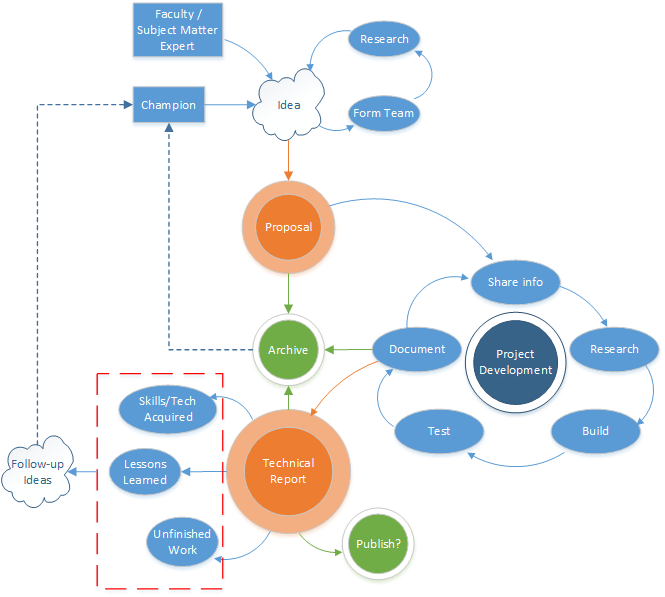
\includegraphics[]{figs/project-life-cycle.png}
%  \caption{Enlarged version of the diagram in \autoref{fig:lifecycle}.}
%\end{figure}

\end{document}
